\documentclass[preprint,12pt]{elsarticle}

\input{preamble.tex}

\journal{Journal of \LaTeX\ template}

\begin{document}

\begin{frontmatter}

\title{HiFiNet: Hierarchical Fault Identification in Wireless Sensor Networks via Edge‑Based Classification and Graph Aggregation}

\author[fidt:pnk]{Nguyen Thi Hanh}
\ead{hanh.nguyenthi@phenikaa-uni.edu.vn}
\author[hust]{Nguyen Tri Nghia}
\ead{nghia.nt215438@sis.hust.edu.vn}
\author[fcs:pnk]{Nguyen Van Son}
\ead{son.nguyenvan@phenikaa-uni.edu.vn}
\author[hust]{Huynh Thi Thanh Binh}
\ead{binhht@soict.hust.edu.vn}
\address[fidt:pnk]{Faculty of Interdisciplinary Digital Technology (FIDT), PHENIKAA University, Vietnam}
\address[hust]{Hanoi University of Science and Technology, Vietnam}
\address[fcs:pnk]{Faculty of Computer Science, PHENIKAA University, Yen Nghia, Ha Dong, Hanoi 12116, Vietnam}

\begin{abstract}
  Wireless Sensor Networks (WSN) are integral to various monitoring applications, but their deployment in harsh environments makes them susceptible to faults, which can compromise data integrity and system reliability. Traditional fault detection methods often struggle to effectively balance accuracy and energy consumption, and they may not fully leverage the complex spatio-temporal correlations inherent in WSN data. In this paper, we introduces HiFiNet, a novel hierarchical fault identification framework that addresses these challenges through a two-stage process. Initially, an edge-based classifier using a Long Short-Term Memory (LSTM) based stacked autoencoder performs temporal feature extraction and preliminary fault screening on individual sensor nodes. Subsequently, a Graph Attention Network (GAT) aggregates information from neighboring nodes, refining the fault diagnosis by considering the broader spatial context. This hierarchical approach, combining edge-based classification with graph aggregation, allows for a comprehensive analysis that captures both local temporal patterns and network-wide spatial dependencies. To validate our approach, we created synthetic WSN datasets by injecting various fault types into real-world environmental data from the Intel Lab Dataset and NASA's MERRA-2 reanalysis data. Experimental results demonstrate that HiFiNet significantly outperforms existing methods in terms of accuracy, F1-score, and precision, showcasing its robustness and effectiveness in identifying diverse fault types. Furthermore, the framework's design allows for a tunable trade-off between diagnostic performance and energy efficiency, making it adaptable to different operational requirements.
\end{abstract}


\begin{keyword}
\textit{Wireless Sensor Networks, Fault Detection, Hierarchical Framework, Graph Attention Network}
\end{keyword}

\end{frontmatter}

\section{Introduction}
Wireless Sensor Networks (WSN) are widely used in a variety of fields such as healthcare, logistics, military, and environment monitoring. These networks, comprised of spatially distributed sensor nodes, support real-time data acquisition and remote monitoring, offering enhanced decision-making and rapid response capabilities in critical scenarios like structural health monitoring and environmental surveillance \cite{Yick2008, Chai2020, Ullo2020}. WSNs are often deployed in harsh and challenging environments where traditional wired solutions are impractical or impossible, ranging from inaccessible terrains, such as in the monitoring of volcanoes or areas with sliding mud, to industrial settings with extreme temperatures, humidity, or vibrations \cite{Gungor2009, Prasad2023}.

This versatility does not come without drawbacks however. The individual sensor nodes are often resource-constrained and operate in unattended conditions, making them highly prone to malfunctions and data corruption. These undetected errors can have severe consequences by generating incorrect predictions, which compromise the reliability of monitoring and control systems and may result in system-wide damage. These reasons explain why a robust fault detection system is crucial. Faults in WSN data are typically categorized based on their temporal behavior (time-based) or their impact on sensor readings (characteristic-based) \cite{Baljak2013, Adday2022}. Figure~\ref{fig:types} depicts the fault types from both perspectives. From a time-based perspective, faults can be classified as soft permanent, intermittent, and transient faults \cite{Prasad2023}. Characteristic-based faults, which describe how the data values themselves are corrupted (e.g., becoming fixed, shifted, or exhibiting other anomalous patterns), also exhibit diverse types according to the literature \cite{Shi2024, Saeed2021, Ni2009, Hasan2024}. While both categorizations are valid, this study concentrates on characteristic-based faults because they provide more direct, actionable insights into the potential root cause. The specific characteristic-based fault types considered in this study will be detailed in our fault taxonomy (see Section~\ref{subsec:types}). Understanding these fault types informs the design of the detection algorithms, which we categorize next.

\begin{figure}
  \centering
  \includegraphics[width=0.8\linewidth]{images/fault_taxonomy.png}
  \caption{WSN Fault Taxonomy}
  \label{fig:types}
\end{figure}

To address the problem of identifying characteristic-based fault types, researchers have employed methods such as model-based approaches, data-driven approaches and hybrid information-based methods \cite{Shi2024}. The most common approach is a model-based algorithm, which utilize mathematical and statistical principles to model each fault type \cite{Panda2014, Ahmad2024}. The data-driven approach on the other hand uses the analysis of data samples obtained to build a model for fault classification \cite{Saeed2021, Prasad2023}. Hybrid information-based methods use both human knowledge and data through a combination of different methods \cite{Sun2023, Shi2024}. Prior work either focuses on temporal patterns at individual nodes or spatial relations across neighbors, but fails to integrate both effectively. However, combining both approaches is crucial, since relying heavily on neighbor-based detection drains nodes’ energy and reduces their lifespans, while using only self-detection methods leads to substantial bias. Therefore, a hierarchical architecture that can effectively model both local temporal dynamics and broader spatial dependencies offers a balanced solution between accuracy and energy consumption. Furthermore, given the complexity of WSN data and the potential for unknown fault patterns, data-driven approaches that can learn from the data themselves are particularly promising. In this work, we investigate the efficacy of a data-driven hierarchical method for WSNs fault diagnosis. The major contribution of this paper are as follows:

\begin{itemize}
  \item Introduce a novel Iterative Graph Network (IGN) that integrates Graph Attention Convolution with a custom Confidence Modulator(CM), dynamically refining node representations through iterative confidence propagation.
  \item Propose HiFiNet, a hierarchical network. HiFiNet first employs a Long Short-Term Memory based stacked autoencoder (LSTM-SAE) at the edge for temporal feature extraction and initial fault screening, followed by IGN for aggregating neighborhood information and refining fault diagnosis.
  \item Simulate real-world fault scenarios by generating synthetic WSN datasets that combines the Intel Lab Dataset measurements \cite{Intel2004} with environmental measurements drawn from NASA’s MERRA‑2 reanalysis data \cite{GMAO2015}.
  \item Evaluate performance including various metrics such as: accuracy, F1-score, precision on the aforementioned datasets, demonstrate improvement against methods in the literature.
\end{itemize}


\section{Literature Review}
Fault diagnosis in WSNs has been extensively studied using both traditional rule-based/statistical methods and machine learning (ML) techniques. In non-ML approaches, sensors often use fixed thresholds, mathematical models, or combinatorial tests to identify anomalies. For example, Panda et al. proposed a fault detection algorithm based on z-score function \cite{Panda2014}. Ahmad et al. proposed Kalman filtering as a lightweight anomaly detector in WSNs, but pure Kalman models degrade under fluctuating conditions \cite{Ahmad2024}. These methods typically require hand-tuned parameters and can yield high false alarms when environmental noise is high \cite{Muhammed2017, Zhang2018}. In contrast, ML-based approaches learn patterns from data. ML methods can automatically capture complex patterns in sensor readings, improving outlier detection without explicit rules. Saeed et al. implemented extremely randomized trees using data collected from Telos B motes and compared against the support vector machine, the multilayer perceptron, the random forest, the decision tree and extra trees \cite{Saeed2021}. ML models often achieve high detection accuracy and F1-scores, but require representative training data and incur higher computational cost.

WSN fault detection architectures are typically classified as centralized, distributed, or self-diagnosis schemes \cite{Takele2024, Prasad2023}. In centralized schemes, all sensor nodes send status reports or readings to a base station (sink), which performs fault analysis \cite{Panda2014}. This simplifies detection logic, but incurs high communication overhead: As the network scales, the sink must process many messages, leading to increased latency and limited real-time applicability \cite{Muhammed2017, Zhang2018}. In contrast, self-diagnosis enables each node to monitor its own status (e.g., battery level or sensor output) and detect local faults. Prasad et al. presented a deep belief network for time-based fault classification using data from each node independently \cite{Prasad2023}. Distributed strategies involve neighbors or cluster-heads collaborating to detect faults. For example, nodes can mutually cross-check readings or vote on anomalies, and cluster-heads can aggregate data for local inference. These decentralized methods improve detection accuracy (errors are confirmed by multiple nodes) and scale better via clustering, but they consume extra energy and bandwidth for peer communication. In particular, Adday et al. note that cluster-based diagnosis can reduce communication relative to flat schemes and improve scalability \cite{Adday2022}.

Recent advances have explored hierarchical and hybrid techniques that fuse multiple levels of analysis and feature types. Hierarchical WSN architectures (e.g. clustering) naturally allow multistage diagnosis, where cluster heads perform local detection and report to higher layers. The hybrid information-based method combines expert knowledge with quantitative data using many different algorithms. Shi et al. used a belief rule base with adaptive attribute weights to improve on the traditional static rule base \cite{Shi2024}. Importantly, this study emphasizes that sensor data possess strong temporal and spatial correlations and that fault features should capture both aspects. These efforts suggest a trend toward spatio-temporal fusion: e.g. using time-series prediction at each node together with spatial neighbor-consensus. Nevertheless, truly integrated models that jointly leverage per-node temporal dynamics and network-wide spatial context are still rare in the literature. HiFiNet is motivated by this gap, seeking to hierarchically combine temporal modeling (autoregressive encoding at nodes) with spatial modeling (graph-based fusion across nodes).


\section{System Model and Problem Statement}
\subsection{System Model}
 We consider a WSN as an undirected graph \(G=(V,E))\), where \(V=\{v_1, v_2, \ldots, v_N\}\) is the set of \(N\) sensor nodes and \(E \subseteq V \times V\) represents bidirectional communication links between neighboring nodes. Each node \(v_i\) is equipped with a sensing modality and generates a time-series measurement \(x_i(t)\) at discrete time steps \(t=1, 2, \ldots, T\). Communication between \(v_i\) and \(v_j\) is possible if \((v_i,v_j) \in E\). Figure~\ref{fig:wsn} depicts the structure of a WSN used in our model.

\begin{figure}
\centering
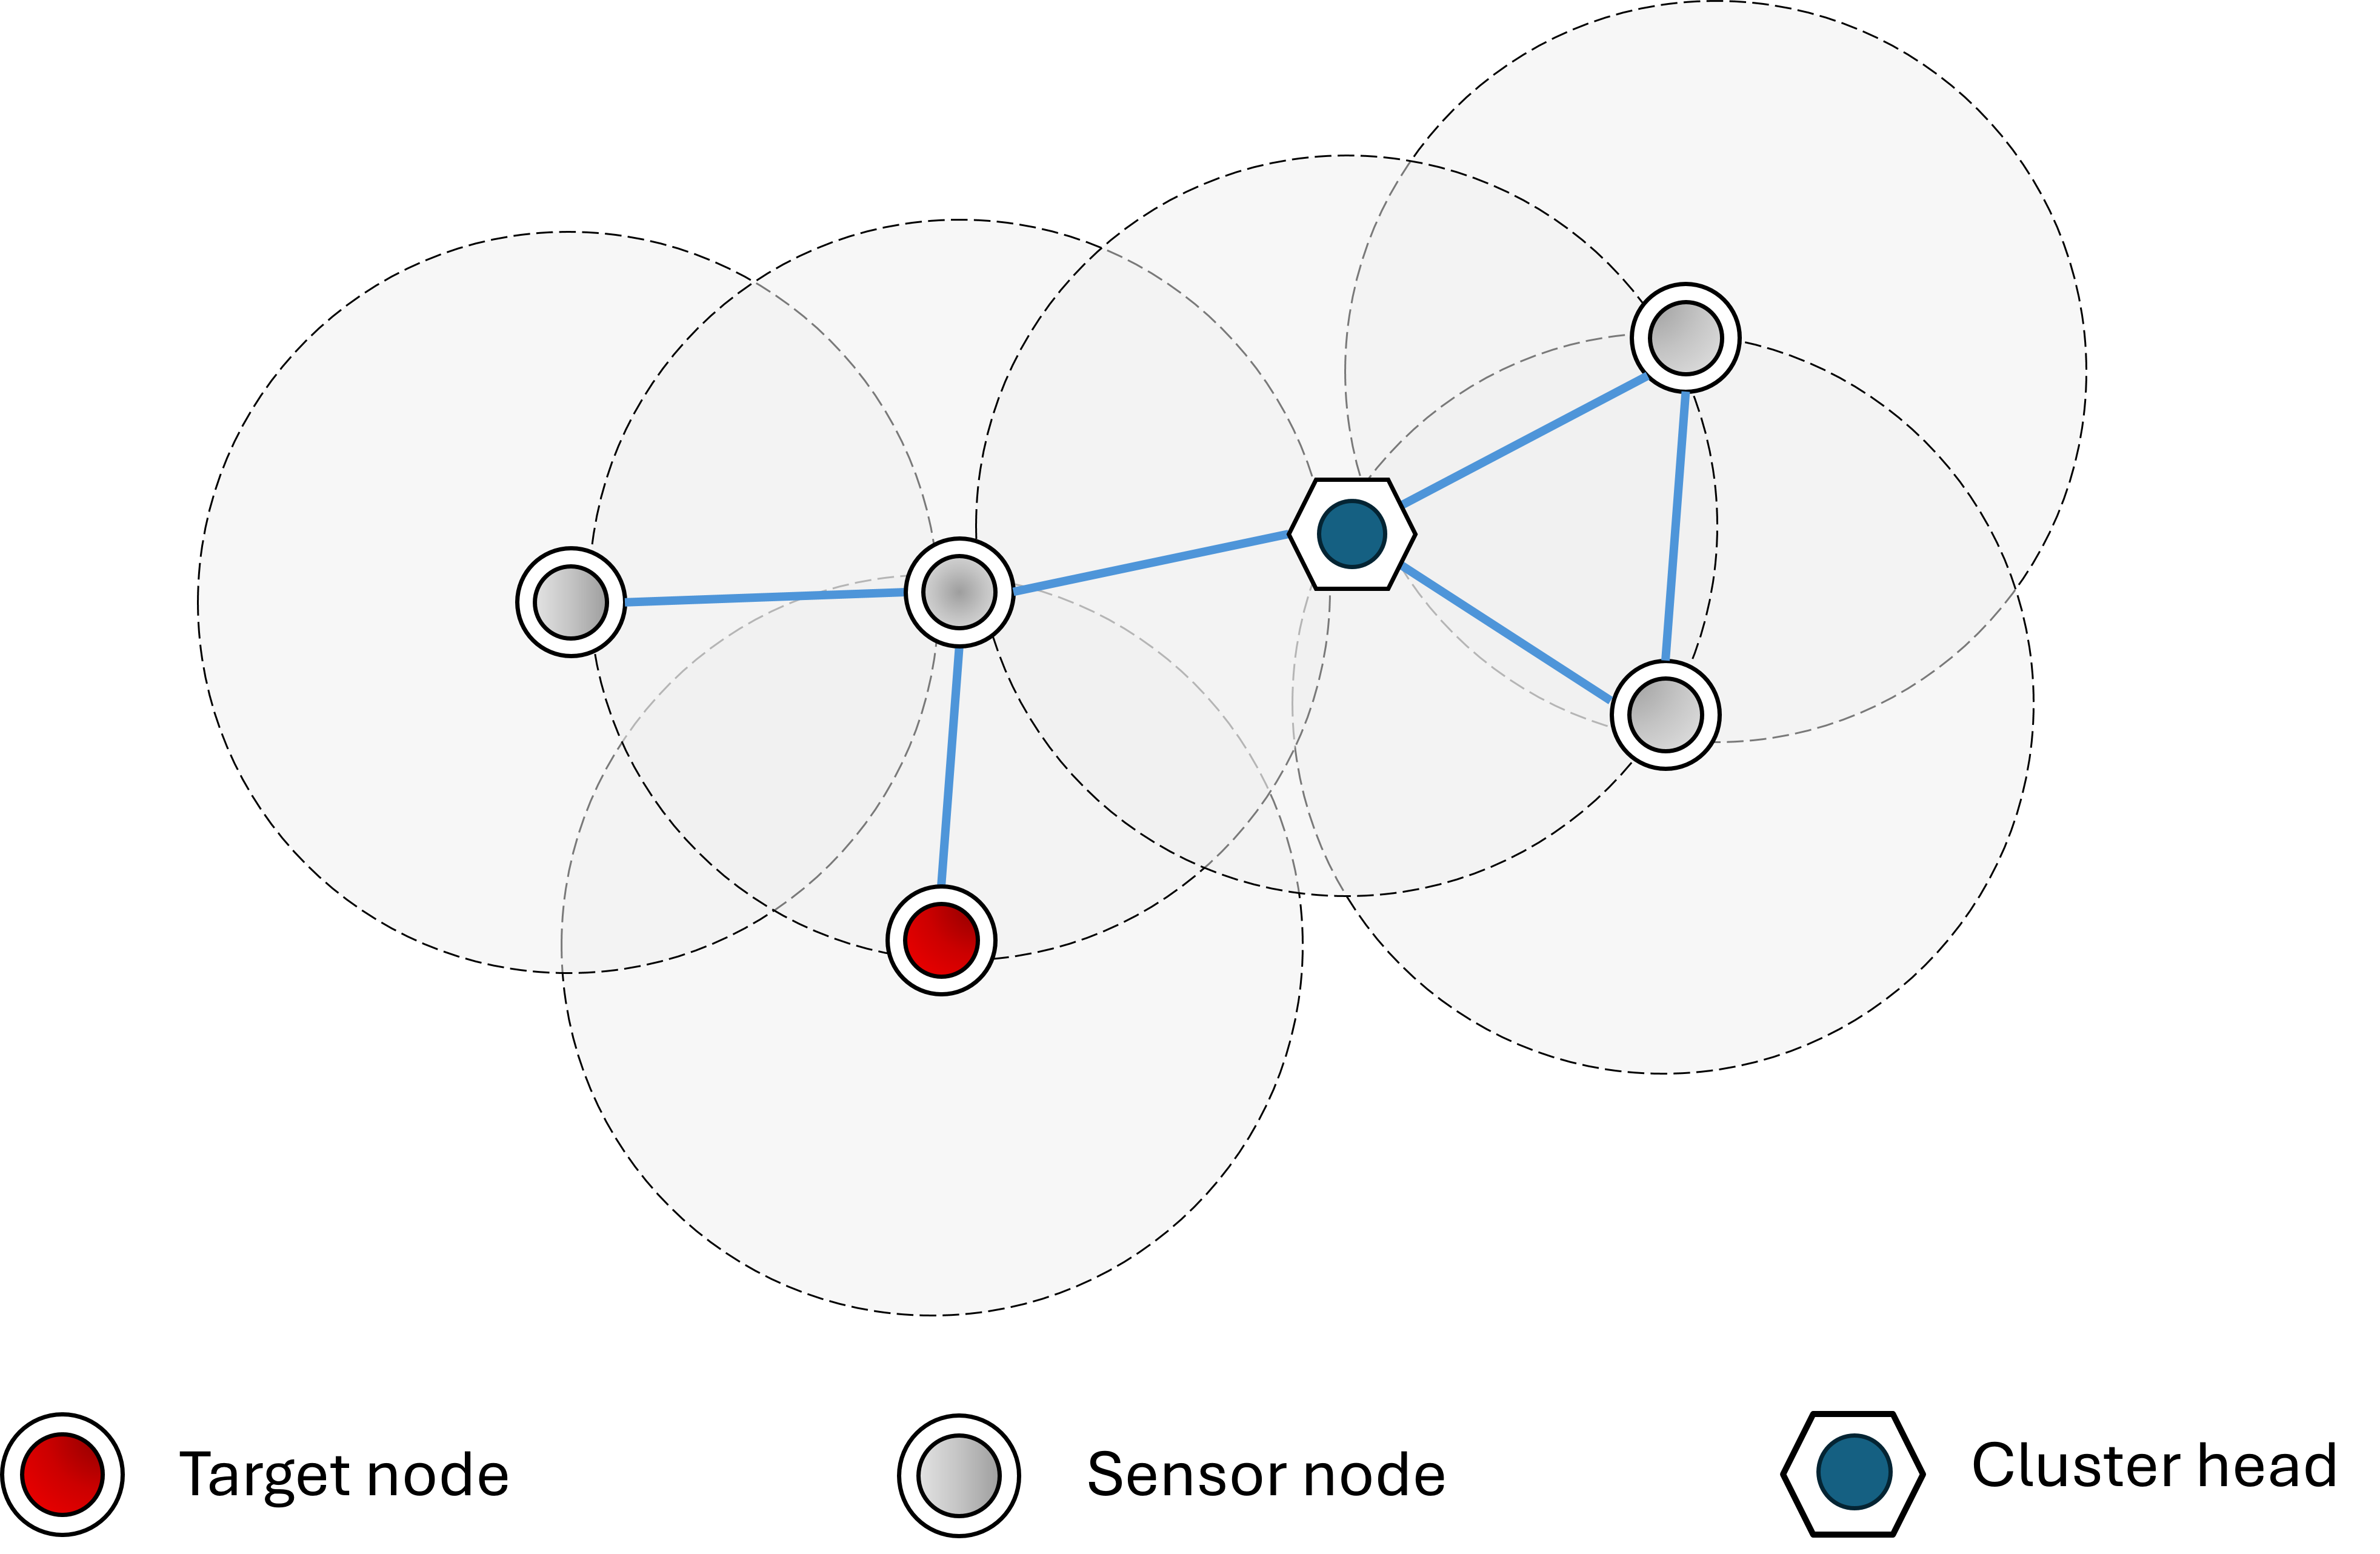
\includegraphics[width=0.8\linewidth]{images/WSN.png}
\caption{Example of a WSN cluster with a base station. Target node is the node which data sequence needed fault classification.}
\label{fig:wsn}
\end{figure}

This paper make the following additional assumptions:
\begin{itemize}
\item Static or Slowly Varying Topology: Sensor nodes are assumed to be stationary or exhibit negligible mobility during the diagnosis window, so that network links \(E\) remain constant or change infrequently.
\item Global Time Synchronization: Nodes maintain loosely synchronized clocks, ensuring measurements \(x_i(t)\) across the network align within a bounded jitter.
\item Existence of a Single High-Capacity Base Node: A base node with higher computation and memory resources is reachable (directly or multi-hop) from all nodes and knows the network topology apriori.
\end{itemize}

\subsection{Problem Statement}
Given a segment of a sensor time series and a predefined set of fault classes, the problem is to assign the most appropriate fault class label to that time series segment.

Consider an input time series \(X_w = (x_t, x_{t+1}, \ldots, x_{t+w-1})\) of length \(w\), where \(x_i \in \mathbb{R}\) is the sensor reading at discrete time step \(i\). Define \(C = \{c_1, c_2, \ldots, c_K\}\) as the set of \(K\) mutually exclusive fault classes as detailed in the fault taxonomy in Section~\ref{subsec:types} and the normal (fault-free) class.

The object is to learn a classification function (or hypothesis) \(h\) that maps the input feature vector \(\mathbf{x}\) (derived from \(X_w\)) to a predicted fault class label \(\hat{y}\ \in C\).

\subsection{Fault Taxonomy}
\label{subsec:types}
Building upon the general categorization of faults, this section details the specific characteristic-based fault types that are the focus of our detection and diagnosis efforts. These faults represent common anomalies observed in the readings of the WSN sensor and are well documented in the literature \cite{Saeed2021, Hasan2024, Shi2024, Ni2009}. The development of robust fault detection algorithm is predicated on a comprehensive understanding of their distinct signatures. The faults considered in this study are hardover, drift, spike, erratic, and stuck-at fault.

\subsubsection{Hardover Fault}
A hardover fault, also commonly referred to as a bias fault, occurs when the sensor's output signal experiences a large, sudden and persistent shift by a constant offset from its normal operational range \cite{Saeed2021, Shi2024, Hasan2024}. The sensor continues to respond to changes in the measured variable, but all readings are offset by this fixed amount. If \(S_\text{normal}(t)\) is the true sensor reading at time \(t\), the faulty signal, \(S_\text{hardover}(t)\), can be represented as:
\begin{equation}
S_\text{hardover}(t) = S_\text{normal}(t) + b,
\label{eq:hardover}
\end{equation}
where \(b \in [5, 10]\) is a constant bias value \cite{Saeed2021}.

\subsubsection{Drift Fault}
A drift fault is characterized by a gradual and continuous deviation of the sensor readings from the true values over time \cite{Saeed2021, Hasan2024}. This deviation often manifests as a linear increase or decrease, though non-linear drifts are also possible. Drift can be caused by aging components, environmental changes affecting the sensor, or gradual degradation of sensor calibration. For a linear drift, the faulty signal, \(S_\text{drift}(t_n)\) at discrete time sample \(n\), can be modeled as:
\begin{equation}
S_\text{drift}(t_n) = S_\text{normal}(t_n) + n \cdot b_0,
\label{eq:drift}
\end{equation}
where \(n\) is the time index or sample number, and \(b_0\) is an initial constant drift rate \cite{Saeed2021}. Hasan et al. also model this as \(S_\text{drift}^N = S_\text{normal}^N +\beta^N\), where \(\beta^N\) represents the accumulated drift \cite{Hasan2024}.

\subsubsection{Spike Fault}
Spike faults are transient anomalies characterized by sudden, short-duration, large-magnitude deviations in sensor readings, after which the readings typically return to normal or near-normal values \cite{Saeed2021, Shi2024}. They appear as sharp peaks or impulses in the data stream. Spikes can be caused by electromagnetic interference, power supply glitches, or other transient disturbances. If \(S_\text{normal}(t)\) is the normal signal, a spike at time \(t_s\) might be represented as:
\begin{equation}
S_\text{spike}(t_s) = S_\text{normal}(t_s) + b_\text{spike},
\label{eq:spike}
\end{equation}
where \(b_\text{spike}\) is a constant large value, and for \(t \neq t_s\): \(S_\text{spike}(t) \approx S_\text{normal}(t)\) \cite{Saeed2021, Shi2024}.

\subsubsection{Erratic Fault}
An erratic fault, sometimes referred to as precision degradation or increased noise, is characterized by sensor readings that exhibit random fluctuations of significantly increased amplitude around the true value \cite{Saeed2021}. While the average reading over a long period might still be close to the true value, the individual readings become highly unreliable due to the increased variance. This can be caused by failing sensor components, loose connections, or severe environmental interference. The faulty signal can be represented as:
\begin{equation}
S_\text{erratic}(t) = S_\text{normal}(t) + \eta(t),
\label{eq:erratic}
\end{equation}
where \(\eta(t)\) is a noise term with zero mean but significantly higher variance (\(\sigma_\text{erratic} \gg \sigma_\text{normal}\)) than the inherent sensor noise under normal operating conditions \cite{Saeed2021}.

\subsubsection{Stuck-at Fault}
A stuck-at fault (or stuck fault) occurs when the sensor output remains fixed at a constant value for a prolonged period, irrespective of any changes in the measured physical phenomenon \cite{Saeed2021, Hasan2024, Shi2024}. This constant value could be zero, a previous valid reading, the maximum or minimum of the sensor's range, or an arbitrary value. Common causes include complete sensor failure, signal clipping, or a disconnection in the data path. Mathematically, this is expressed as:
\begin{equation}
S_\text{stuck} = c,
\label{eq:stuck}
\end{equation}
where \(c\) is a constant value, either from the nearest normal value or a random value \cite{Saeed2021, Hasan2024, Shi2024}.


\section{Proposed Algorithm}
\label{sec:method}
Our goal is to detect and label faults in wireless sensor networks (WSNs) from each node’s time-series data and its spatial context. The expected output is a fault label (or “normal”) for every data segment.

We propose HiFiNet, a Hierarchical Fault Identification Network, for the classification of sensor faults in WSNs. HiFiNet jointly leverages per-node temporal features and network‐level interactions to outperform single-level baselines. Moving beyond conventional approaches, our key innovations lie in the novel integration of a confidence-guided Graph Attention Network. This architecture establishes a new paradigm for fault diagnosis by dynamically learning to trust and weigh information from individual sensors and the broader network context. We will demonstrate how this sophisticated approach leads to a more robust and accurate fault identification system with the ability to balance between performance and energy consumption. The overall inference pipeline is depicted in Figure~\ref{fig:hifinet}.

\begin{figure}
  \centering
  \includegraphics[width=0.8\linewidth]{images/HiFiNet.png}
  \caption{Proposed HiFiNet inference pipeline, illustrating the Edge Classifier processing a target node's temperature sequence and the Network Classifier integrating edge outputs with contextual network data.}
  \label{fig:hifinet}
\end{figure}

\subsection{Edge Classifier}
The first stage of HiFiNet is the Edge Classifier. This component's primary role is to analyze the time-series data from an individual target sensor node. Through this analysis, it extracts discriminative features and performs an initial fault classification. The design of the Edge Classifier involves a two-phase training process. It begins with the unsupervised pre-training of a feature extractor, which is based on the LSTM-SAE architecture. This is followed by a supervised fine-tuning phase for the fault classification task. The specifics of this training methodology are detailed in \ref{app:edge_training}. The edge logits and the learned embedding are then forwarded to the network layer to serve as the initial node states, denoted as \(\mathcal{H}^{(0)}\).

\subsection{Iterative Graph Network}
The second stage of HiFiNet is the IGN, which refines the initial fault assessments or embeddings from the Edge Classifier by incorporating network-wide spatial context and inter-node dependencies. The core of the Network Classifier is an IGN. Figure~\ref{fig:ign} depicts the information flow in an IGN.

\begin{figure}
  \centering
  \includegraphics[width=0.8\linewidth]{images/IGN.png}
  \caption{Illustration of the Iterative Graph Network architecture, showing the iterative process of feature modulation, graph attention convolution, and confidence update.}
  \label{fig:ign}
\end{figure}

The IGN is designed to dynamically refine node representations by iteratively propagating and aggregating information across the graph, modulated by an evolving confidence measure. Let \(\mathcal{H}^{(0)} \in \mathbb{R}^{N \times d_0}\) be the vector representation of a node with \(N\) is the number of nodes and \(d_0\) is the dimension of the edge output. The IGN performs \(K\) iterations.

In each iteration \(k = 0, \dots, K\):
\begin{itemize}
  \item Feature Modulation (for \(k > 0\)):
    The initial node embeddings \(\mathbf{H}^{(0)}\) are modulated based on a confidence score vector \(\mathbb{c}^{(k-1)} \in \mathbb{R}^{N \times 1}\), derived from the \((k-1)\)-th iteration's GAT output. A Confidence Modulator function, \(\mathcal{M}_{\text{c}}\), is employed using Feature-wise Linear Modulation (FiLM):
    \begin{equation}
      \mathcal{H}'^{(k)} = \mathcal{M}_{\text{c}}(\mathcal{H}^{(0)}, \mathbb{c}^{(k-1)}) = g_{\gamma}(c^{(k-1)}) \odot \mathcal{H}^{(0)} + g_{\beta}(c^{(k-1)})
    \end{equation}
    where \(g_{\gamma}(\cdot)\) and \(g_{\beta}(\cdot)\) are learnable functions that generate scaling and shifting parameters from the confidence scores, and \(\odot\) denotes element-wise multiplication. For the first iteration \(k=0\), no modulation is applied, so \(\mathcal{H}'^{(0)} = \mathcal{H}^{(0)}\). The Confidence Modulator allows the network to adaptively emphasize or de-emphasize features based on the current confidence in their classification.

  \item Graph Attention Convolution (GAT) Block:
    The modulated features \(\mathbb{H}'^{(k)}\) are then processed by a GAT block, denoted as \(\mathcal{G}\). This block typically consists of one or more Graph Attention Convolution layers, which enable nodes to selectively attend to their neighbors' features when updating their own representations:
    \begin{equation}
      \mathcal{H}_{\text{G}}^{(k)} = \mathcal{G}(\mathcal{H}'^{(k)}, A)
    \end{equation}
    where \(A\) is the adjacency matrix representing the graph structure. Each GAT layer computes attention coefficients for neighboring nodes, aggregates their features weighted by these coefficients, and applies a linear transformation. Layer normalization and activation functions  are often applied between GAT layers. Dropout are also used for regularization. The output \(\mathcal{H}_{\text{G}}^{(k)} \in \mathbb{R}^{N \times d_{\text{G}}}\) contains node representations that have incorporated information from their local graph neighborhood.

  \item Temporary Classification and Confidence Update (if \(k < K-1)\):
    If it is not the final iteration, the output \(\mathcal{H}_{\text{G}}^{(k)}\) is passed through a temporary classifier, \(f_{\text{temp}}\), to obtain intermediate class logits \(z^{(k)}\) for each node:
    \begin{equation}
      z^{(k)} = f_{\text{temp}}(\mathcal{H}_{\text{G}}^{(k)})
    \end{equation}
    These logits are converted to probabilities \(P^{(k)}\) using the softmax function:
    \begin{equation}
      P^{(k)} = \text{softmax}(\mathbf{z}^{(k)})
    \end{equation}
    The confidence score \(c_i^{(k)}\) for each node \(i\) is then derived from these probabilities, typically as the maximum probability value:
    \begin{equation}
      c_i^{(k)} = \max(P_i^{(k)})
    \end{equation}
    This results in a confidence vector \(\mathbf{c}^{(k)}\), which is then used in the Feature Modulation step of the next iteration (\(k+1\)). This iterative process allows the model to progressively refine its understanding by focusing subsequent GAT operations based on the certainty of intermediate predictions.
\end{itemize}

After \(K\) iterations, the final GAT output \(\mathcal{H}_{\text{G}}^{(K_{iter}-1)}\) represents the spatially-refined node embeddings. This and the original representation are then passed to a classification head to output the network classification. At inference, only the encoder and the IGN forward pass is needed, the reconstruction branch is omitted.


\section{Experiments and Result}
In this section, we evaluated our proposed method against other methods in the literature. From previous research about fault diagnosis in WSNs, we selected  Deep Belief Network \cite{Prasad2023}, LSTM-AE \cite{Khan2024}, and Support Vector Machine(SVM).

\subsection{Dataset}
For purpose of fault detection, we created an original dataset using data from NASA MERRA-2 reanalysis data (Temperature at 2 Meter) as substitution for measurements taken from a WSN \cite{GMAO2015}. The data is collected from the North Vietnam region from a period of roughly 6 months. Another dataset used for performance evaluation is the Intel Lab Dataset. This dataset comprises readings from a network of 54 sensor nodes, specifically Mica2Dot devices, which were outfitted with environmental sensing capabilities. These nodes systematically captured time-stamped information relating to ambient conditions, including temperature, humidity, light levels, and the sensors' own voltage. The data acquisition process occurred at intervals of roughly 31 seconds for each sensor. The collection period for this particular dataset extended from late February 2004 through early April 2004 \cite{Intel2004}.

\subsection{Fault Injection}
A key challenge in developing fault detection systems in WSNs is the scarcity of real-world fault data, making it difficult to test a model's robustness. Therefore, to evaluate the performance of HiFiNet in realistic environment, synthetic faults were injected into the pre-processed normal temperature data.

For each experimental dataset used, six node is chosen as a representative of a typical cluster (\(n \approx 6\)). Each node is injected only one type of fault to isolate the influence of each fault on the sensor readings. This setup allows for the analysis of one specific fault type per sensor in the context of other faulty and normal sensors.

Multiple datasets were generated with varying overall percentages of faulty instances, specifically 5\%, 10\%, 15\%, and 20\% of the total data points being faulty. Analysis of real world data have shown \(<20\%\) readings faults in WSNs. Within each dataset, the total fault rate was divided equally among the five predefined fault types. Faults were injected based on their mathematical models Equation \ref{eq:hardover}, \ref{eq:drift}, \ref{eq:spike}, \ref{eq:erratic}, and \ref{eq:stuck}. In total, 4 datasets are created from each original dataset corresponding to each fault rate.

The process for injecting fault to the dataset involves three main steps:
\begin{itemize}
    \item Filter the original dataset by chosen nodes and time range
    \item Fault rate and the appropriate fault type are chosen for each node
    \item Inject fault to each sample using Equation \ref{eq:hardover}, \ref{eq:drift}, \ref{eq:spike}, \ref{eq:erratic}, and \ref{eq:stuck}
\end{itemize}
A sequence is assigned a specific fault type's label if \textbf{any} single sample within its window of length \(w\) contains that corresponding fault. Otherwise, if no sample within the sequence contains any fault, it is labeled as 'normal'.

\subsection{Metrics}
To evaluate the performance of the proposed HiFiNet and compare it with other methods, several standard classification metrics are employed. These metrics are calculated based on the number of true positives (TP), false positives (FP), true negatives (TN), and false negatives (FN) for each class. In a multi-class classification problem, these are often computed for each class $c_i$ in a set of classes $C = \{c_1, c_2, \dots, c_K\}$.

Given that \(TP_i\) is the number of true positives for class \(c_i\), \(FP_i\) is the number of false positives for class \(c_i\), \(FN_i\) is the number of false negatives for class \(c_i\), \(N\) is the total number of instances, \(N_i\) is the number of true instances belonging to class \(c_i\).

Accuracy measures the overall correctness of the classifier. It is the ratio of the number of correctly classified instances to the total number of instances.
\begin{equation}
  \text{Accuracy} = \frac{\sum_{i=1}^{K} TP_i}{N}
\end{equation}

Next, precision measures the proportion of positively predicted instances for class \(c_i\) that were actually correct. It is calculated as the ratio of true positives for class \(c_i\) to the sum of true positives and false positives for class \(c_i\).
\begin{equation}
  \text{Precision}_i = \frac{TP_i}{TP_i + FP_i}
\end{equation}
The weighted average precision is computed as:
\begin{equation}
  \text{Weighted Precision} = \sum_{i=1}^{K} \left( \frac{N_i}{N} \times \text{Precision}_i \right)
\end{equation}

Finally, the F1-score is the harmonic mean of precision and recall for a class \(c_i\), providing a single score that balances both concerns.
\begin{equation}
  \text{F1-score}_i = 2 \times \frac{\text{Precision}_i \times \text{Recall}_i}{\text{Precision}_i + \text{Recall}_i}
\end{equation}
Similarly, the weighted average F1-score is calculated by:
\begin{equation}
  \text{Weighted F1-score} = \sum_{i=1}^{K} \left( \frac{N_i}{N} \times \text{F1-score}_i \right)
\end{equation}

\subsection{Experiment Settings}
The experiment was conducted with the following parameters:
\begin{itemize}
  \item Test period: 2024-05-24 to 2024-07-01 (MERRA-2), 2004-03-06 to 2004-03-07 (Intel)
  \item \(w = 24\)
  \item \(b_\text{hardover}\ = 5\)
  \item \(b_\text{drift} = 0.3\)
  \item \(b_\text{spike} = 3\)
  \item \(\eta_\text{erratic} = 2\eta_\text{normal}\)
\end{itemize}

All experiment is implemented in Python and run inside Kaggle Notebook with a P100 GPU.

\subsection{Evaluation Result}
We now verify the two claims in Section~\ref{sec:method}: (i) edge-to-graph synergy, (ii) energy-aware tunability. The overall classification accuracy, shown in Figure~\ref{fig:accuracy}, demonstrates a substantial uplift from HiFiNet. HiFiNet maintains a \(2\sim6\%\) accuracy advantage over the second-best model LSTM-AE. SVM and DBN lag behind with sub \(90\%\) and sub \(80\%\) accuracies respectively across datasets. More importantly, the accuracy of HiFiNet does not degrade significantly as fault rate increases when compared to other methods. This indicates that information from neighbors collected in HiFiNet has a major impact in stabilizing the performance when noise becomes more prevalent

\begin{figure}
  \centering
  \includegraphics[width=\linewidth]{images/accuracy.png}
  \caption{Accuracy versus Fault Rate comparison between HiFiNet and other methods.}
  \label{fig:accuracy}
\end{figure}

To conduct further analysis into each method's discriminative performance, Figure~\ref{fig:pr_curve} plots Precision Recall curve at the highest stress level (20\% fault rate). The results clearly indicate that the HiFiNet model substantially outperforms the other methods, achieving an AUPRC of 0.927. Its curve dominates the others, maintaining high precision (above 0.95) for recall values up to approximately 0.8. The next best performing model is the LSTM-SAE, with an AUPRC of 0.719, followed by the SVM at 0.659 and the DBN at 0.590. Overall, the HiFiNet architecture demonstrates a superior balance of precision and recall for this classification task.

\begin{figure}
  \centering
  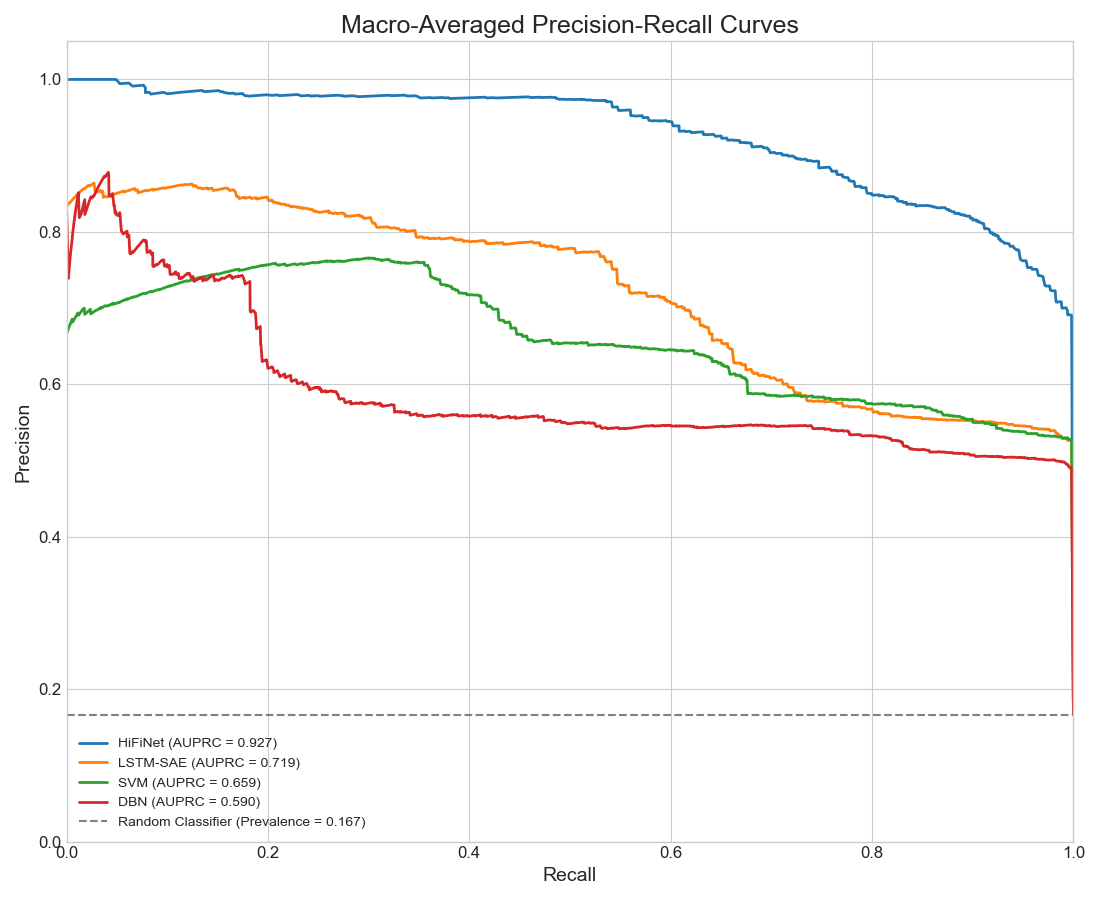
\includegraphics[width=\linewidth]{images/pr_curve.png}
  \caption{Precision-Recall curves comparison between HiFiNet and other methods on Intel 20\% dataset.}
  \label{fig:pr_curve}
\end{figure}

Next, Figure~\ref{fig:f1_drop} provides a direct, quantitative measure of model stability. It visualizes the absolute drop in F1-Score as the fault rate increases from 5\% to 20\%. A smaller bar indicates greater robustness against worsening data quality. HiFiNet clearly stands out with the smallest performance drop on both datasets (2.06 points for MERRA-2 and 3.93 for INTEL). In contrast, models like SVM and LSTM-AE experience much larger drops, exceeding 11 and 12 points, respectively. This bar chart offers a stark visual confirmation of HiFiNet's superior stability and reliability under varying conditions.

\begin{figure}
  \centering
  \includegraphics[width=\linewidth]{images/f1_drop.png}
  \caption{F1-Score drop comparison between HiFiNet and other methods.}
  \label{fig:f1_drop}
\end{figure}

To further analyze HiFiNet's performance on a granular level, Figure~\ref{fig:confusion_matrix} provides the confusion matrix of the model. HiFiNet demonstrates high accuracy for several categories, correctly identifying the majority of instances for Normal, Hardover, Drift and Spike classes. However, performance on Stuck-at fault remains less than desirable with 42 misclassifications out of 175 samples. The model also has struggles with identifying Erratic fault with almost half of the instance in the class being misclassifications.

\begin{figure}
  \centering
  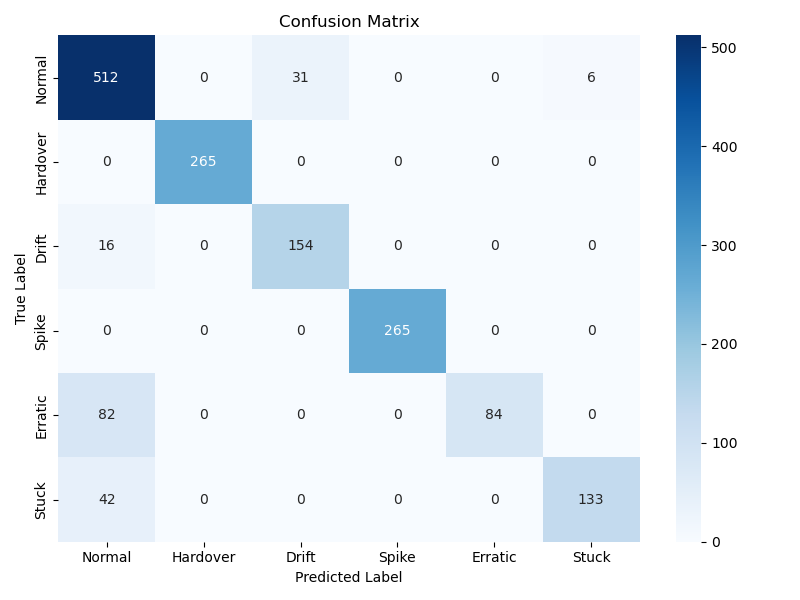
\includegraphics[width=\linewidth]{images/confusion_matrix.png}
  \caption{Confusion Matrix of HiFiNet on Intel 20\% dataset.}
  \label{fig:confusion_matrix}
\end{figure}

While the previous figures provide a visual analysis of key performance trends, the complete numerical results for all metrics are consolidated in Table~\ref{tab:metrics} for reference. In addition, a case study on the individual classification of HiFiNet is conducted in Section~\ref{case:classification}.

\begin{table}
  \centering
  \resizebox{\linewidth}{!}{%
    \begin{tabular}{@{}llrrrrrrrr@{}}
      \toprule
      & & \multicolumn{4}{c}{MERRA-2} & \multicolumn{4}{c}{INTEL} \\
      \cmidrule(lr){3-6} \cmidrule(lr){7-10}
      Metric & Model & 5\% & 10\% & 15\% & 20\% & 5\% & 10\% & 15\% & 20\% \\
      \midrule
      \multirow{4}{*}{Accuracy}
      & HiFiNet   & \textbf{95.20} & \textbf{94.66} & \textbf{93.23} & \textbf{92.78} & \textbf{93.08} & \textbf{90.75} & \textbf{89.50} & \textbf{88.87} \\
      & LSTM-AE   & 93.42 & 91.49 & 89.46 & 86.07 & 90.44 & 87.11 & 83.40 & 77.42 \\
      & SVM       & 88.63 & 85.05 & 82.27 & 78.68 & 87.16 & 83.77 & 79.24 & 70.06 \\
      & DBN       & 76.95 & 73.60 & 68.82 & 69.42 & 85.09 & 75.34 & 76.28 & 72.01 \\
      \midrule
      \multirow{4}{*}{F1-Score}
      & HiFiNet   & \textbf{94.70} & \textbf{94.49} & \textbf{93.12} & \textbf{92.64} & \textbf{92.32} & \textbf{89.50} & \textbf{88.99} & \textbf{88.39} \\
      & LSTM-AE   & 92.04 & 90.68 & 88.68 & 85.37 & 88.39 & 84.66 & 82.32 & 75.77 \\
      & SVM       & 86.62 & 81.68 & 79.64 & 75.43 & 81.57 & 78.19 & 71.89 & 62.30 \\
      & DBN       & 70.72 & 62.89 & 58.39 & 52.60 & 76.02 & 63.65 & 63.65 & 64.39 \\
      \midrule
      \multirow{4}{*}{Precision}
      & HiFiNet   & \textbf{95.21} & \textbf{94.52} & \textbf{93.55} & \textbf{92.89} & \textbf{92.55} & \textbf{91.76} & \textbf{90.16} & \textbf{90.32} \\
      & LSTM-AE   & 92.10 & 90.90 & 89.35 & 85.55 & 89.53 & 86.63 & 82.71 & 76.28 \\
      & SVM       & 86.95 & 82.78 & 81.62 & 79.20 & 76.89 & 73.96 & 67.30 & 69.08 \\
      & DBN       & 70.47 & 60.98 & 53.12 & 59.14 & 72.43 & 66.77 & 57.48 & 65.95 \\
      \bottomrule
    \end{tabular}
  }
  \caption{Comprehensive performance metrics of each method on all datasets.}
  \label{tab:metrics}
\end{table}

\subsection{Ablation Study: Accuracy Tradeoff versus Energy Efficiency of HiFiNet}
This analysis investigates the crucial trade-off between the accuracy gained by incorporating neighborhood data and the energy consumed in the process, a primary concern in resource-constrained WSNs. The study's goal is to provide insight into how HiFiNet can be configured for different operational requirements, balancing diagnostic performance with network lifetime.

To quantify the energy cost, we adopt a widely used energy model for WSNs. The model accounts for the energy dissipated during signal transmission, reception, and processing. The combined energy for receiving, aggregating and transmitting data from node \(i\) to node \(j\) is defined by:
\begin{equation}
  E_{t_{ij}} = l (\epsilon_{elec} + \epsilon_{da} + \epsilon_{fs} \cdot d^2_{ij}),
\end{equation}
where \(d_{ij}\) is the distance between nodes \(i\) and \(j\), \(l\) is the number of bits, and \(\epsilon_{elec}\), \(\epsilon_{fs}\), and \(\epsilon_{da}\) represent the energy per bit dissipated in the electronic circuitry of the transmitter or the receiver, the energy cost of transmitting one bit of data over a unit distance squared at short distance, and the energy to aggregate one bit of data.

In our model, we use standard parameter values where \(\epsilon_{elec} = 50\) \si{nJ/bit}, \(\epsilon_{fs} = 10\) \si{pJ/bit/m^2}, \(\epsilon_{mp} = 0.0013\) \si{pJ/bit/m^4}, and the data aggregation energy cost \(\epsilon_{da} = 5 \) \si{nJ/bit}. We define Energy Efficiency (EE) as the inverse of the total energy spent:
\begin{equation}
  EE = 1 / E_{total}.
\end{equation}

The ablation study compares the full HiFiNet architecture against its baseline component: the Edge Classifier operating in isolation (i.e., without the Network Classifier's spatial aggregation). The Accuracy Delta (\%) measures the performance improvement provided by the full HiFiNet over this baseline. We introduce a tunable parameter, Time Delay \(t\), which represents the frequency of execution for the Network Classifier. A time delay of \(t=0\) means the spatial aggregation is performed for every time window processed by the Edge Classifier. A delay of \(t=k\) means the aggregation is performed only once every \(k+1\) time windows. The network is assumed to adopt the Constrained Application Protocol (CoAP) with a transmission overhead of 32 bytes.

The results of this trade-off are presented in Figure~\ref{fig:accuracy_tradeoff}. At a time delay of \(t=0\), the system performs continuous spatial aggregation. This yields the maximum diagnostic benefit, with HiFiNet achieving an Accuracy Delta of over \(3.1\%\) compared to the edge-only model. This configuration, however, is the most energy-intensive, resulting in the lowest Energy Efficiency (approx. 40 units).

\begin{figure}
  \centering
  \includegraphics[width=\textwidth]{images/accuracy_tradeoff.png}
  \caption{Accuracy Delta and Energy Efficiency versus Time Delay.  Accuracy Delta represents the performance gain from using the Network Classifier compared to the Edge Classifier alone. Energy Efficiency is inversely proportional to the energy consumed by the communication process.}
  \label{fig:accuracy_tradeoff}
\end{figure}

Conversely, as the Time Delay \(t\) increases, the Network Classifier runs less frequently, drastically reducing the cumulative energy cost. This is reflected in the sharp, monotonic rise of the Energy Efficiency curve, which increases by more than rapidly goes from 0 to 11. This energy saving comes at the cost of accuracy. Since the spatial context is updated less often, its influence diminishes, causing the Accuracy Delta to fall,  and it becomes marginal for \(t > 8\).

This analysis reveals that the system's configuration can be optimized based on deployment needs. For critical applications where maximum accuracy is paramount, a low time delay (\(t=0\) or \(t=1\)) is ideal. However, for long-term monitoring where network longevity is the primary concern, a higher time delay (\(t\ge4\)) can provide substantial energy savings with a modest drop in performance. The region between \(t=1\) and \(t=3\) represents a compelling trade-off where a significant portion of the accuracy gain (1.1\%-1.6\%) is retained while achieving a 2-3 times improvement in energy efficiency over the most aggressive configuration. This demonstrates the flexibility of the HiFiNet architecture, allowing operators to tune the model to strike the right balance between diagnostic accuracy and operational lifetime.

\subsection{Case Study: A Comparative Analysis of HiFiNet Classifications}
\label{case:classification}
To offer a more qualitative understanding of HiFiNet's classification capabilities, this section presents a case study that contrasts its performance with the baseline LSTM-AE on specific fault instances. The analysis centers on two distinct examples of drift fault sequences and the corresponding t-SNE visualizations of the models' learned hidden layer representations.

Figure~\ref{fig:classifications} provides two examples of drift sequences in the dataset. The second sequence displays a classic, gradual, and near-linear increase in temperature readings over time. In contrast, the first sequence presents a more complex and realistic scenario. It is characterized by an initial upward drift that is then interrupted by erratic fluctuations and a sudden drop. This type of non-linear, noisy drift is significantly more challenging to distinguish from normal operational variance. In this particular case, HiFiNet was able to correctly predict the classification of both sequences while LSTM-AE mistakes the sequences to be both from Normal class.

\begin{figure}
    \centering
    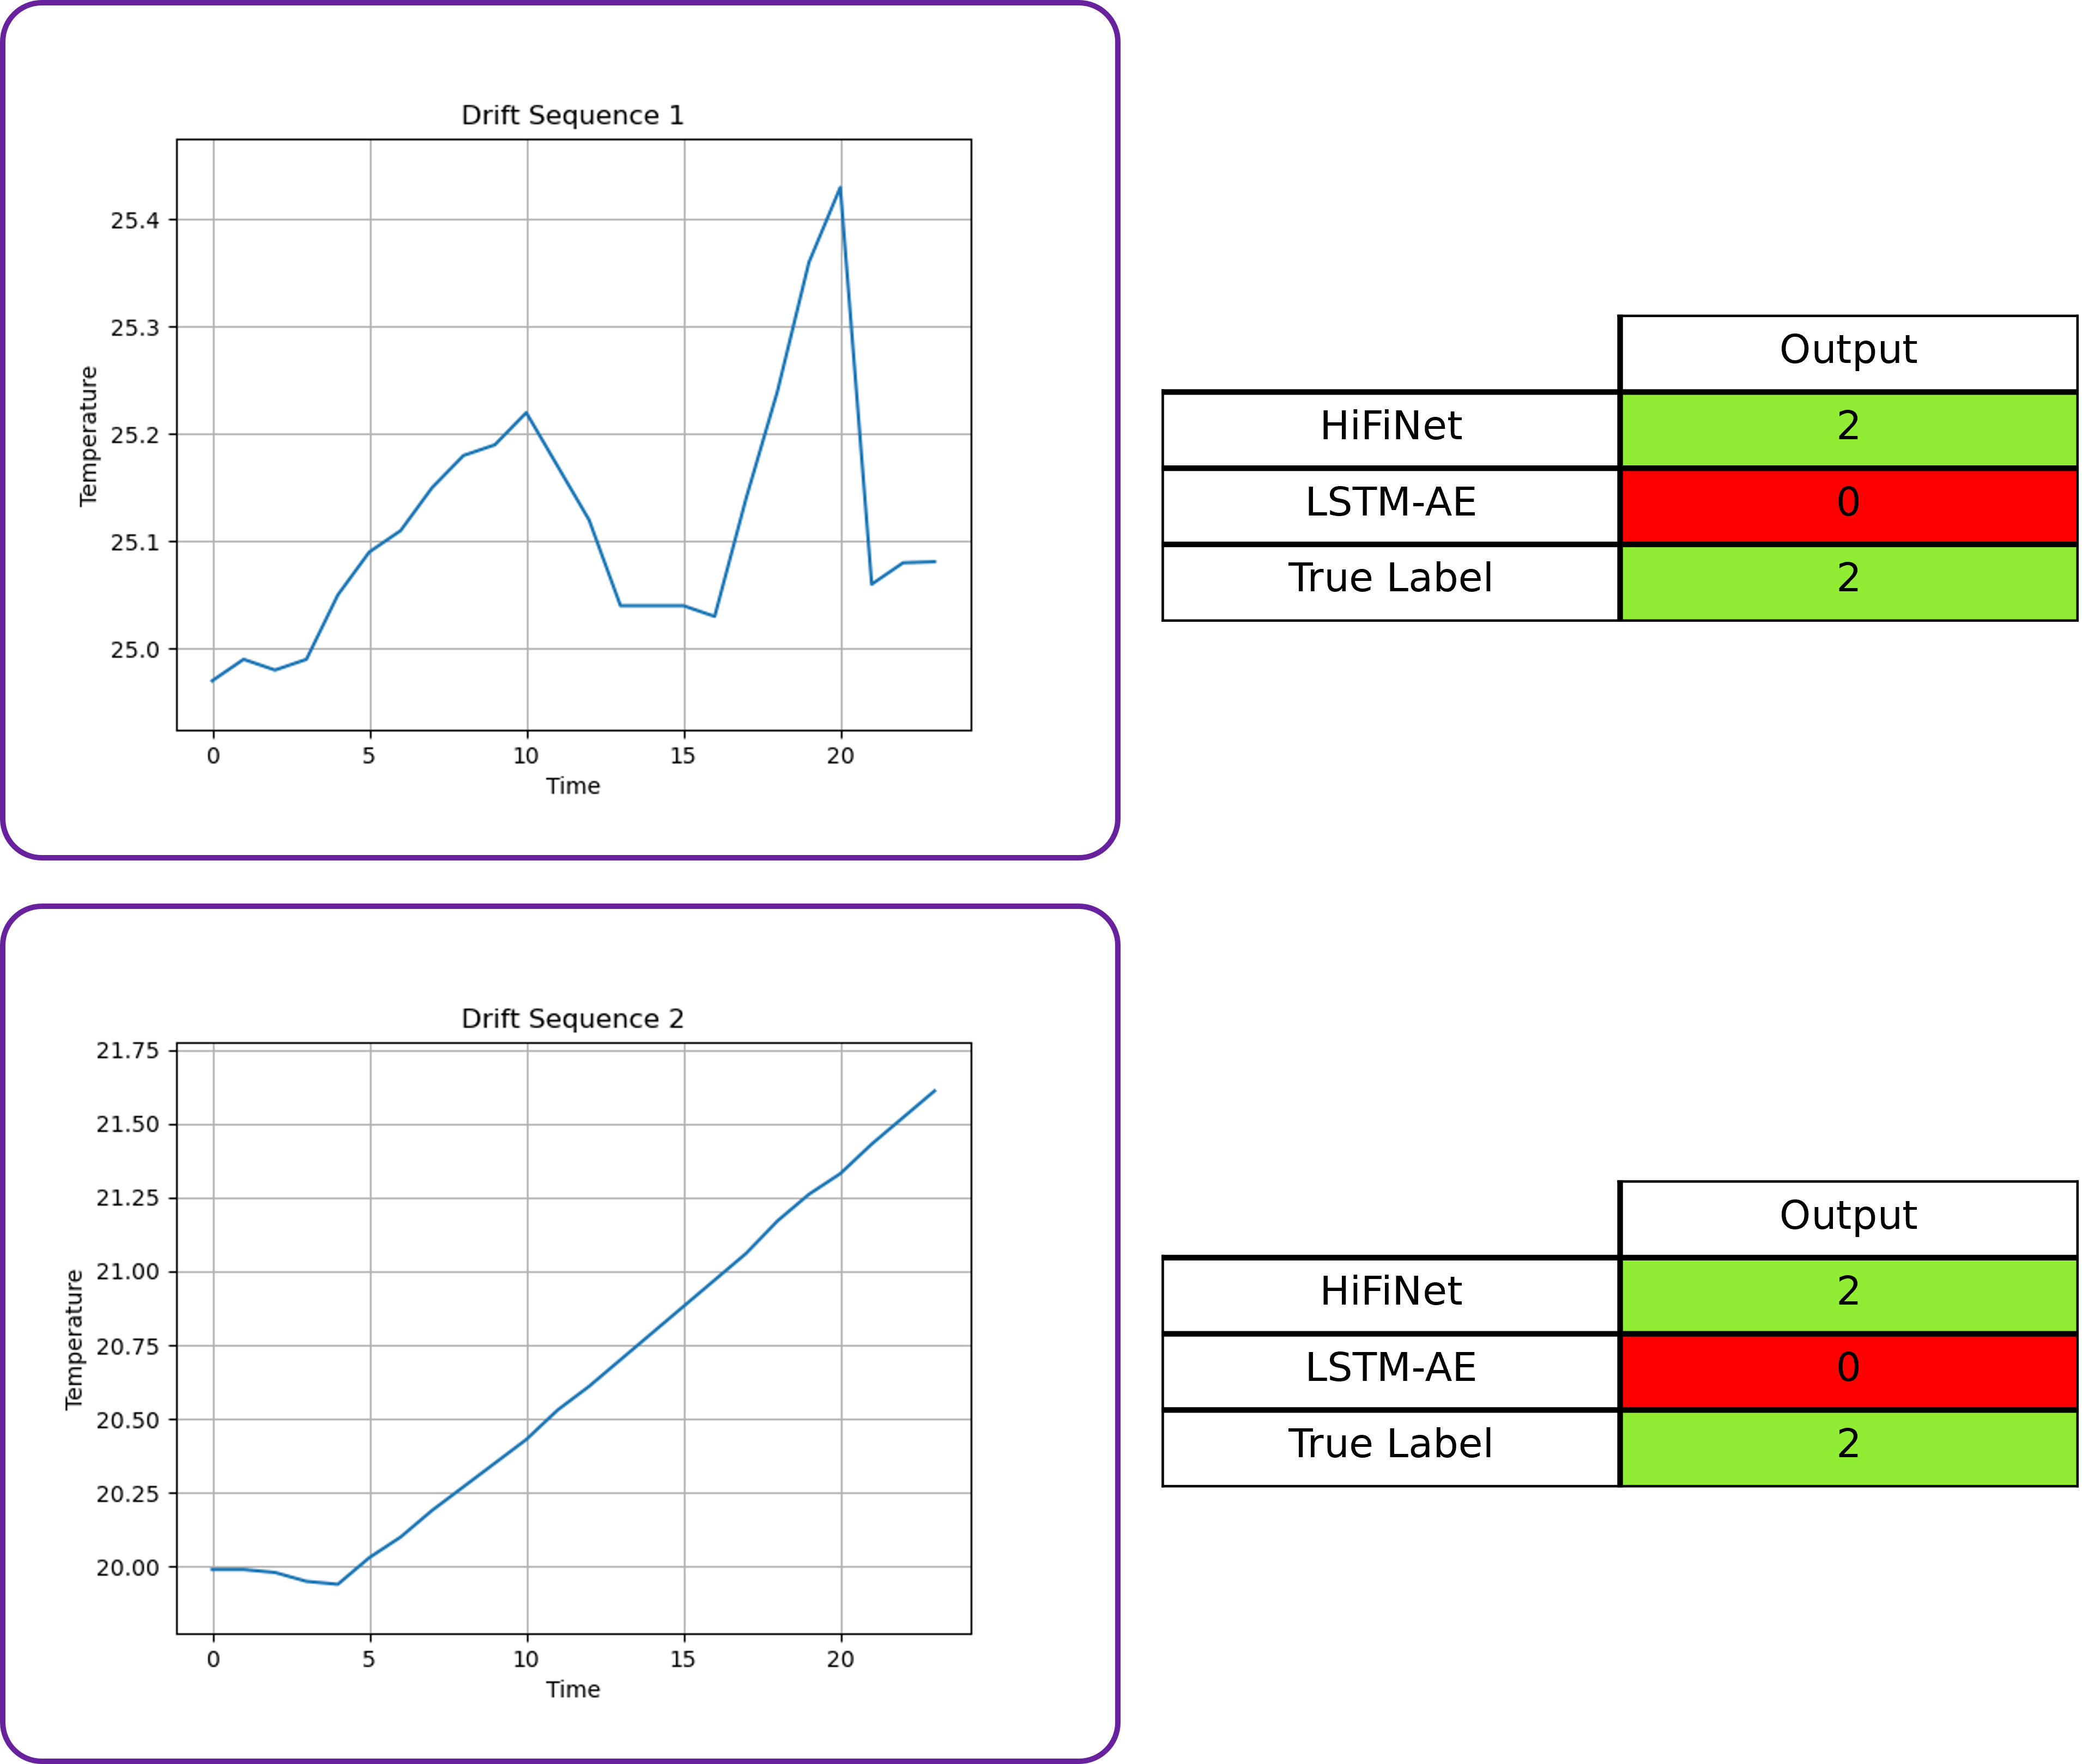
\includegraphics[width=\linewidth]{images/classifications.png}
    \caption{Examples of drift fault sequences in the test dataset and the models predictions.}
    \label{fig:classifications}
\end{figure}

Figure~\ref{fig:tsne} sheds some light into this performance discrepancies of the two models by utilizing t-SNE method. For the LSTM-AE model, the visualization reveals significant confusion between the two classes. The representations of Normal (blue) and Drift (red) data are heavily interspersed, with no clear boundary separating them. Clusters are ill-defined, and many drift instances are scattered amidst normal data points, and vice-versa. The t-SNE plot for HiFiNet, however, tells a different story. The blue dots, representing Normal data, are concentrated in several distinct, dense clusters. This clear demarcation indicates that HiFiNet learns highly discriminative representations. The Drift data itself forms a tight, coherent cluster with little contamination, suggesting that the model effectively captures the unique signature of this fault type, even when presented with noisy and non-linear examples. This enhanced separability demonstrates that HiFiNet's hierarchical approach, which combines temporal analysis with spatial context from neighboring nodes, allows it to form a more robust and abstract representation of what constitutes a "drift". It can look beyond simple linear trends to identify the underlying anomalous behavior, a capability that leads to more accurate and reliable fault diagnosis in complex, real-world scenarios.

\begin{figure}
    \centering
    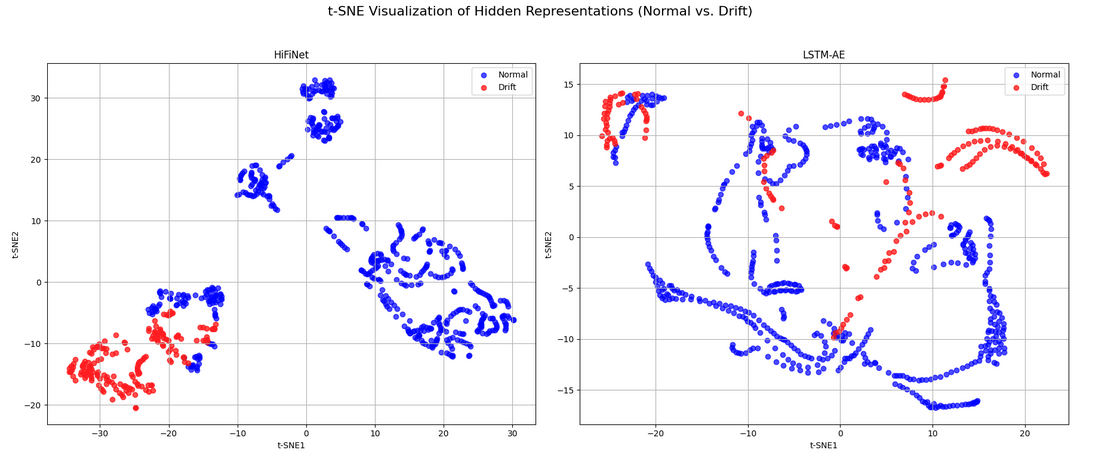
\includegraphics[width=\linewidth]{images/tsne.png}
    \caption{t-SNE visualization of both models hidden representations of the sequences before the classification layer.}
    \label{fig:tsne}
\end{figure}


\section{Conclusion}
In this paper, we have presented HiFiNet, a hierarchical fault identification network for Wireless Sensor Networks that synergistically combines edge-based classification with graph aggregation. By first analyzing temporal data at the individual node level and then refining the diagnosis through a graph attention mechanism that incorporates spatial context from neighboring nodes, HiFiNet achieves a new level of accuracy and robustness in fault detection. Our comprehensive experiments, conducted on realistic datasets with injected faults, have demonstrated the superiority of HiFiNet over methods such as DBN, LSTM-AE, and SVM. The results show a significant improvement in key performance metrics, including accuracy, F1-score, and precision, across various fault types and rates. Notably, HiFiNet exhibits greater stability as noise and data quality issues increase, a critical advantage in real-world WSN deployments. A tunable mechanism unique to HiFiNet was also explored which demonstrated the model ability to balance accuracy and power consumption.

Future work could explore the adaptation of HiFiNet to dynamic network topologies and the inclusion of a wider range of fault types. Additionally, the implementation of the proposed model on actual WSN hardware would provide further insights into its real-world performance and energy consumption. Overall, HiFiNet represents a significant advancement in the field of fault diagnosis for WSNs, offering a powerful and adaptable solution for ensuring data integrity and reliability in a wide array of applications.


\clearpage
\bibliography{references.bib}

\clearpage
\appendix
\section{Edge Classifier Training}
\label{app:edge_training}
The design of the Edge Classifier involves a two-phase training process: unsupervised pre-training of a feature extractor using a LSTM-SAE architecture, followed by supervised fine-tuning for the fault classification task.

The feature-extraction component is built from an LSTM-SAE with encoder layers. In the first phase, this autoencoder is trained in an unsupervised, layer-wise fashion to learn compressed representations of \(X_w\). Define \(E_l(\cdot; \theta_{E_l})\) as the \(l\)-th LSTM encoder layer with parameters \(\theta_{E_l}\), \(D_l(\cdot; \theta_{D_l})\) as the corresponding decoder layer with parameters \(\theta_{D_l}\), and \(H_l\) as the hidden representation output by \(E_l\). We have:
\begin{itemize}
  \item \emph{Layer \(l=1\):}
    \begin{equation}
      \begin{aligned}
        H_1 &= E_1(X_w; \theta_{E_1}), \\
        \hat X_w &= D_1(H_1; \theta_{D_1}), \\
      \end{aligned}
    \end{equation}
    with \(\hat X_w\) being the reconstructed input. Then the objective is to optimize the reconstruction loss with respective to the network parameters:
    \begin{equation}
      (\hat \theta_{E_1},\,\hat \theta_{D_1}) = \underset{\theta_{E_1}, \theta_{D_1}} {\arg\min} \mathcal L_{\text{recon}}(X_w; \hat X_w)
    \end{equation}
  \item \emph{Layer \(l = 2, \ldots, L\)}

    Define \(H^*_{l-1}\) as the output of the \((l-1)\)-th trained encoder layer. We have:
    \begin{equation}
      \begin{aligned}
        H_l &= E_l(H^*_{L-1}; \theta_{E_l}), \\
        \hat H^*_{l-1} &= D_l(H_l; \theta_{D_l}), \\
      \end{aligned}
    \end{equation}
    with \(\hat H^*_{l-1}\) being the reconstructed input. Again the objective is to optimize the reconstruction loss with to the network parameters:
    \begin{equation}
      (\hat \theta_{E_l},\,\hat \theta_{D_l}) = \underset{\theta_{E_l}, \theta_{D_l}} {\arg\min} \mathcal L_{\text{recon}}(H^*_{l-1}; \hat H^*_{l-1})
    \end{equation}
\end{itemize}
After all \(L\) layers are pre-trained, the full stacked LSTM encoder is formed by concatenating these trained layers: \(E_\text{stacked}(\cdot; \Theta^*_{E}) = E_L(\ldots E_1(\cdot; \theta^*_{E_L}) \ldots;\theta^*_{E_L})\)

The pre-trained stacked LSTM encoder, \(E_\text{stacked}\), now served as the feature extractor for the Edge Classifier. In the second phase, classification head is attached to this encoder to create the Edge Classifier. The complete network is then trained using the labeled dataset. The edge logits and embedding are forwarded to the network layer as initial node states \(\mathcal{H}^{(0)}\).

\end{document}
